% This file is generated by the MATLAB m-file laprint.m. It can be included
% into LaTeX documents using the packages graphicx, color and psfrag.
% It is accompanied by a postscript file. A sample LaTeX file is:
%    \documentclass{article}\usepackage{graphicx,color,psfrag}
%    \begin{document}% This file is generated by the MATLAB m-file laprint.m. It can be included
% into LaTeX documents using the packages graphicx, color and psfrag.
% It is accompanied by a postscript file. A sample LaTeX file is:
%    \documentclass{article}\usepackage{graphicx,color,psfrag}
%    \begin{document}% This file is generated by the MATLAB m-file laprint.m. It can be included
% into LaTeX documents using the packages graphicx, color and psfrag.
% It is accompanied by a postscript file. A sample LaTeX file is:
%    \documentclass{article}\usepackage{graphicx,color,psfrag}
%    \begin{document}% This file is generated by the MATLAB m-file laprint.m. It can be included
% into LaTeX documents using the packages graphicx, color and psfrag.
% It is accompanied by a postscript file. A sample LaTeX file is:
%    \documentclass{article}\usepackage{graphicx,color,psfrag}
%    \begin{document}\input{mrmse_det_300}\end{document}
% See http://www.mathworks.de/matlabcentral/fileexchange/loadFile.do?objectId=4638
% for recent versions of laprint.m.
%
% created by:           LaPrint version 3.16 (13.9.2004)
% created on:           09-Apr-2014 02:43:05
% eps bounding box:     15 cm x 11.25 cm
% comment:              
%
\begin{psfrags}%
\psfragscanon%
%
% text strings:
\psfrag{s09}[t][t]{\color[rgb]{0,0,0}\setlength{\tabcolsep}{0pt}\begin{tabular}{c}$\log_2 (M) + 1$\end{tabular}}%
\psfrag{s10}[b][b]{\color[rgb]{0,0,0}\setlength{\tabcolsep}{0pt}\begin{tabular}{c}MRMSE\end{tabular}}%
\psfrag{s14}[][]{\color[rgb]{0,0,0}\setlength{\tabcolsep}{0pt}\begin{tabular}{c} \end{tabular}}%
\psfrag{s15}[][]{\color[rgb]{0,0,0}\setlength{\tabcolsep}{0pt}\begin{tabular}{c} \end{tabular}}%
\psfrag{s16}[l][l]{\color[rgb]{0,0,0}SLF}%
\psfrag{s17}[l][l]{\color[rgb]{0,0,0}EKF}%
\psfrag{s18}[l][l]{\color[rgb]{0,0,0}UKF}%
\psfrag{s19}[l][l]{\color[rgb]{0,0,0}CKF}%
\psfrag{s20}[l][l]{\color[rgb]{0,0,0}SLF}%
%
% xticklabels:
\psfrag{x01}[t][t]{0}%
\psfrag{x02}[t][t]{0.1}%
\psfrag{x03}[t][t]{0.2}%
\psfrag{x04}[t][t]{0.3}%
\psfrag{x05}[t][t]{0.4}%
\psfrag{x06}[t][t]{0.5}%
\psfrag{x07}[t][t]{0.6}%
\psfrag{x08}[t][t]{0.7}%
\psfrag{x09}[t][t]{0.8}%
\psfrag{x10}[t][t]{0.9}%
\psfrag{x11}[t][t]{1}%
\psfrag{x12}[t][t]{4.5}%
\psfrag{x13}[t][t]{5}%
\psfrag{x14}[t][t]{5.5}%
\psfrag{x15}[t][t]{6}%
\psfrag{x16}[t][t]{6.5}%
\psfrag{x17}[t][t]{7}%
\psfrag{x18}[t][t]{7.5}%
\psfrag{x19}[t][t]{8}%
\psfrag{x20}[t][t]{8.5}%
\psfrag{x21}[t][t]{9}%
%
% yticklabels:
\psfrag{v01}[r][r]{0}%
\psfrag{v02}[r][r]{0.1}%
\psfrag{v03}[r][r]{0.2}%
\psfrag{v04}[r][r]{0.3}%
\psfrag{v05}[r][r]{0.4}%
\psfrag{v06}[r][r]{0.5}%
\psfrag{v07}[r][r]{0.6}%
\psfrag{v08}[r][r]{0.7}%
\psfrag{v09}[r][r]{0.8}%
\psfrag{v10}[r][r]{0.9}%
\psfrag{v11}[r][r]{1}%
\psfrag{v12}[r][r]{0}%
\psfrag{v13}[r][r]{0.005}%
\psfrag{v14}[r][r]{0.01}%
\psfrag{v15}[r][r]{0.015}%
%
% Figure:
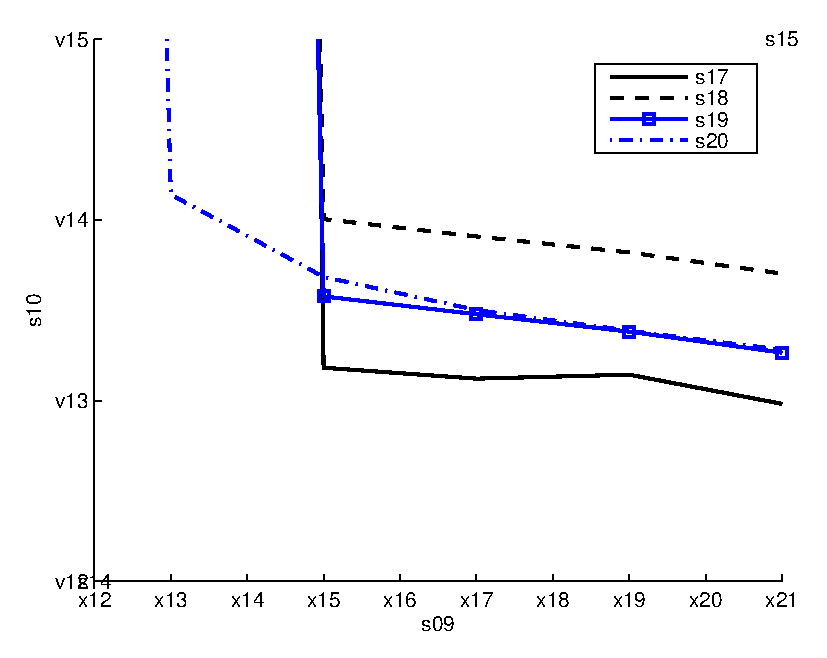
\includegraphics[width=15cm]{mrmse_det_300.eps}%
\end{psfrags}%
%
% End mrmse_det_300.tex
\end{document}
% See http://www.mathworks.de/matlabcentral/fileexchange/loadFile.do?objectId=4638
% for recent versions of laprint.m.
%
% created by:           LaPrint version 3.16 (13.9.2004)
% created on:           09-Apr-2014 02:43:05
% eps bounding box:     15 cm x 11.25 cm
% comment:              
%
\begin{psfrags}%
\psfragscanon%
%
% text strings:
\psfrag{s09}[t][t]{\color[rgb]{0,0,0}\setlength{\tabcolsep}{0pt}\begin{tabular}{c}$\log_2 (M) + 1$\end{tabular}}%
\psfrag{s10}[b][b]{\color[rgb]{0,0,0}\setlength{\tabcolsep}{0pt}\begin{tabular}{c}MRMSE\end{tabular}}%
\psfrag{s14}[][]{\color[rgb]{0,0,0}\setlength{\tabcolsep}{0pt}\begin{tabular}{c} \end{tabular}}%
\psfrag{s15}[][]{\color[rgb]{0,0,0}\setlength{\tabcolsep}{0pt}\begin{tabular}{c} \end{tabular}}%
\psfrag{s16}[l][l]{\color[rgb]{0,0,0}SLF}%
\psfrag{s17}[l][l]{\color[rgb]{0,0,0}EKF}%
\psfrag{s18}[l][l]{\color[rgb]{0,0,0}UKF}%
\psfrag{s19}[l][l]{\color[rgb]{0,0,0}CKF}%
\psfrag{s20}[l][l]{\color[rgb]{0,0,0}SLF}%
%
% xticklabels:
\psfrag{x01}[t][t]{0}%
\psfrag{x02}[t][t]{0.1}%
\psfrag{x03}[t][t]{0.2}%
\psfrag{x04}[t][t]{0.3}%
\psfrag{x05}[t][t]{0.4}%
\psfrag{x06}[t][t]{0.5}%
\psfrag{x07}[t][t]{0.6}%
\psfrag{x08}[t][t]{0.7}%
\psfrag{x09}[t][t]{0.8}%
\psfrag{x10}[t][t]{0.9}%
\psfrag{x11}[t][t]{1}%
\psfrag{x12}[t][t]{4.5}%
\psfrag{x13}[t][t]{5}%
\psfrag{x14}[t][t]{5.5}%
\psfrag{x15}[t][t]{6}%
\psfrag{x16}[t][t]{6.5}%
\psfrag{x17}[t][t]{7}%
\psfrag{x18}[t][t]{7.5}%
\psfrag{x19}[t][t]{8}%
\psfrag{x20}[t][t]{8.5}%
\psfrag{x21}[t][t]{9}%
%
% yticklabels:
\psfrag{v01}[r][r]{0}%
\psfrag{v02}[r][r]{0.1}%
\psfrag{v03}[r][r]{0.2}%
\psfrag{v04}[r][r]{0.3}%
\psfrag{v05}[r][r]{0.4}%
\psfrag{v06}[r][r]{0.5}%
\psfrag{v07}[r][r]{0.6}%
\psfrag{v08}[r][r]{0.7}%
\psfrag{v09}[r][r]{0.8}%
\psfrag{v10}[r][r]{0.9}%
\psfrag{v11}[r][r]{1}%
\psfrag{v12}[r][r]{0}%
\psfrag{v13}[r][r]{0.005}%
\psfrag{v14}[r][r]{0.01}%
\psfrag{v15}[r][r]{0.015}%
%
% Figure:
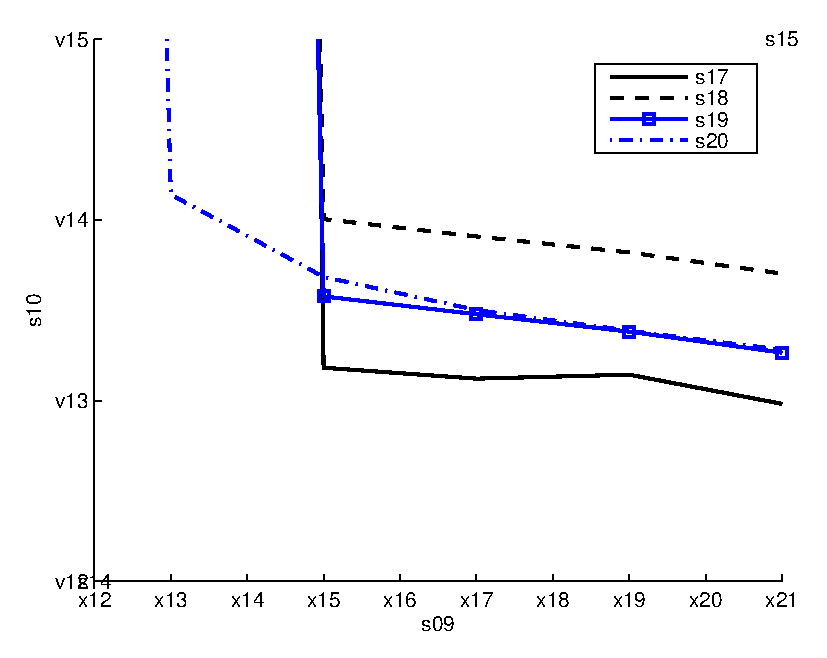
\includegraphics[width=15cm]{mrmse_det_300.eps}%
\end{psfrags}%
%
% End mrmse_det_300.tex
\end{document}
% See http://www.mathworks.de/matlabcentral/fileexchange/loadFile.do?objectId=4638
% for recent versions of laprint.m.
%
% created by:           LaPrint version 3.16 (13.9.2004)
% created on:           09-Apr-2014 02:43:05
% eps bounding box:     15 cm x 11.25 cm
% comment:              
%
\begin{psfrags}%
\psfragscanon%
%
% text strings:
\psfrag{s09}[t][t]{\color[rgb]{0,0,0}\setlength{\tabcolsep}{0pt}\begin{tabular}{c}$\log_2 (M) + 1$\end{tabular}}%
\psfrag{s10}[b][b]{\color[rgb]{0,0,0}\setlength{\tabcolsep}{0pt}\begin{tabular}{c}MRMSE\end{tabular}}%
\psfrag{s14}[][]{\color[rgb]{0,0,0}\setlength{\tabcolsep}{0pt}\begin{tabular}{c} \end{tabular}}%
\psfrag{s15}[][]{\color[rgb]{0,0,0}\setlength{\tabcolsep}{0pt}\begin{tabular}{c} \end{tabular}}%
\psfrag{s16}[l][l]{\color[rgb]{0,0,0}SLF}%
\psfrag{s17}[l][l]{\color[rgb]{0,0,0}EKF}%
\psfrag{s18}[l][l]{\color[rgb]{0,0,0}UKF}%
\psfrag{s19}[l][l]{\color[rgb]{0,0,0}CKF}%
\psfrag{s20}[l][l]{\color[rgb]{0,0,0}SLF}%
%
% xticklabels:
\psfrag{x01}[t][t]{0}%
\psfrag{x02}[t][t]{0.1}%
\psfrag{x03}[t][t]{0.2}%
\psfrag{x04}[t][t]{0.3}%
\psfrag{x05}[t][t]{0.4}%
\psfrag{x06}[t][t]{0.5}%
\psfrag{x07}[t][t]{0.6}%
\psfrag{x08}[t][t]{0.7}%
\psfrag{x09}[t][t]{0.8}%
\psfrag{x10}[t][t]{0.9}%
\psfrag{x11}[t][t]{1}%
\psfrag{x12}[t][t]{4.5}%
\psfrag{x13}[t][t]{5}%
\psfrag{x14}[t][t]{5.5}%
\psfrag{x15}[t][t]{6}%
\psfrag{x16}[t][t]{6.5}%
\psfrag{x17}[t][t]{7}%
\psfrag{x18}[t][t]{7.5}%
\psfrag{x19}[t][t]{8}%
\psfrag{x20}[t][t]{8.5}%
\psfrag{x21}[t][t]{9}%
%
% yticklabels:
\psfrag{v01}[r][r]{0}%
\psfrag{v02}[r][r]{0.1}%
\psfrag{v03}[r][r]{0.2}%
\psfrag{v04}[r][r]{0.3}%
\psfrag{v05}[r][r]{0.4}%
\psfrag{v06}[r][r]{0.5}%
\psfrag{v07}[r][r]{0.6}%
\psfrag{v08}[r][r]{0.7}%
\psfrag{v09}[r][r]{0.8}%
\psfrag{v10}[r][r]{0.9}%
\psfrag{v11}[r][r]{1}%
\psfrag{v12}[r][r]{0}%
\psfrag{v13}[r][r]{0.005}%
\psfrag{v14}[r][r]{0.01}%
\psfrag{v15}[r][r]{0.015}%
%
% Figure:
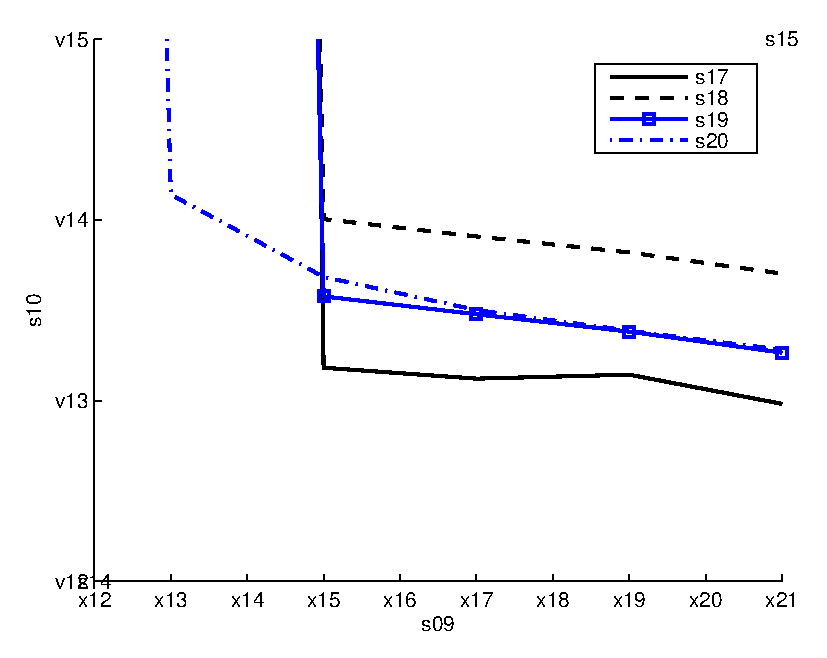
\includegraphics[width=15cm]{mrmse_det_300.eps}%
\end{psfrags}%
%
% End mrmse_det_300.tex
\end{document}
% See http://www.mathworks.de/matlabcentral/fileexchange/loadFile.do?objectId=4638
% for recent versions of laprint.m.
%
% created by:           LaPrint version 3.16 (13.9.2004)
% created on:           09-Apr-2014 02:43:05
% eps bounding box:     15 cm x 11.25 cm
% comment:              
%
\begin{psfrags}%
\psfragscanon%
%
% text strings:
\psfrag{s09}[t][t]{\color[rgb]{0,0,0}\setlength{\tabcolsep}{0pt}\begin{tabular}{c}$\log_2 (M) + 1$\end{tabular}}%
\psfrag{s10}[b][b]{\color[rgb]{0,0,0}\setlength{\tabcolsep}{0pt}\begin{tabular}{c}MRMSE\end{tabular}}%
\psfrag{s14}[][]{\color[rgb]{0,0,0}\setlength{\tabcolsep}{0pt}\begin{tabular}{c} \end{tabular}}%
\psfrag{s15}[][]{\color[rgb]{0,0,0}\setlength{\tabcolsep}{0pt}\begin{tabular}{c} \end{tabular}}%
\psfrag{s16}[l][l]{\color[rgb]{0,0,0}SLF}%
\psfrag{s17}[l][l]{\color[rgb]{0,0,0}EKF}%
\psfrag{s18}[l][l]{\color[rgb]{0,0,0}UKF}%
\psfrag{s19}[l][l]{\color[rgb]{0,0,0}CKF}%
\psfrag{s20}[l][l]{\color[rgb]{0,0,0}SLF}%
%
% xticklabels:
\psfrag{x01}[t][t]{0}%
\psfrag{x02}[t][t]{0.1}%
\psfrag{x03}[t][t]{0.2}%
\psfrag{x04}[t][t]{0.3}%
\psfrag{x05}[t][t]{0.4}%
\psfrag{x06}[t][t]{0.5}%
\psfrag{x07}[t][t]{0.6}%
\psfrag{x08}[t][t]{0.7}%
\psfrag{x09}[t][t]{0.8}%
\psfrag{x10}[t][t]{0.9}%
\psfrag{x11}[t][t]{1}%
\psfrag{x12}[t][t]{4.5}%
\psfrag{x13}[t][t]{5}%
\psfrag{x14}[t][t]{5.5}%
\psfrag{x15}[t][t]{6}%
\psfrag{x16}[t][t]{6.5}%
\psfrag{x17}[t][t]{7}%
\psfrag{x18}[t][t]{7.5}%
\psfrag{x19}[t][t]{8}%
\psfrag{x20}[t][t]{8.5}%
\psfrag{x21}[t][t]{9}%
%
% yticklabels:
\psfrag{v01}[r][r]{0}%
\psfrag{v02}[r][r]{0.1}%
\psfrag{v03}[r][r]{0.2}%
\psfrag{v04}[r][r]{0.3}%
\psfrag{v05}[r][r]{0.4}%
\psfrag{v06}[r][r]{0.5}%
\psfrag{v07}[r][r]{0.6}%
\psfrag{v08}[r][r]{0.7}%
\psfrag{v09}[r][r]{0.8}%
\psfrag{v10}[r][r]{0.9}%
\psfrag{v11}[r][r]{1}%
\psfrag{v12}[r][r]{0}%
\psfrag{v13}[r][r]{0.005}%
\psfrag{v14}[r][r]{0.01}%
\psfrag{v15}[r][r]{0.015}%
%
% Figure:
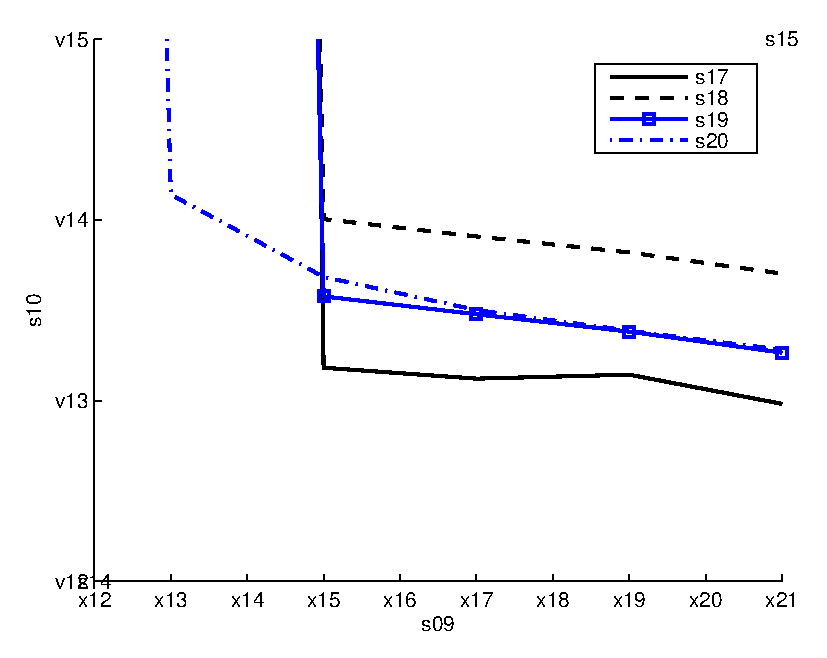
\includegraphics[width=15cm]{mrmse_det_300.eps}%
\end{psfrags}%
%
% End mrmse_det_300.tex
